\section{Lecture 11: Fluid Dynamics}

\subsection{Intermezzo: Concepts from Analysis III}

\begin{eqbox}{Reynolds Transport Theorem Notation}
$$  \int_{CS} \rho \vec{v} (\vec{v} \cdot \hat{n}) \, dA + \int_{CV} \frac{\partial}{\partial t} (\rho \vec{v}) \, dV = \int_{CV} \rho \left( \frac{\partial \vec{v}}{\partial t} + \vec{v} \cdot \nabla \vec{v} \right) dV$$
\end{eqbox}

\subsubsection{I) Einstein Notation}

\textbf{Cartesian Coordinates:}

\begin{center}
\begin{tikzpicture}[scale=1.2, >=stealth]
    \draw[->, thick] (0,0,0) -- (2,0,0) node[right] {$x_2$ (y)};
    \draw[->, thick] (0,0,0) -- (0,2,0) node[above] {$x_3$ (z)};
    \draw[->, thick] (0,0,0) -- (0,0,2) node[below left] {$x_1$ (x)};
    
    \draw[->, primary, thick] (0,0,0) -- (1,0,0) node[midway, below] {$\hat{e}_2$};
    \draw[->, primary, thick] (0,0,0) -- (0,1,0) node[midway, left] {$\hat{e}_3$};
    \draw[->, primary, thick] (0,0,0) -- (0,0,1) node[midway, right] {$\hat{e}_1$};
\end{tikzpicture}
\end{center}

Cartesian vectors: 
$$ \vec{v} = v_x \hat{e}_x + v_y \hat{e}_y + v_z \hat{e}_z = v_1 \hat{e}_1 + v_2 \hat{e}_2 + v_3 \hat{e}_3 $$
$$ \vec{v} = \sum_{i=1}^3 v_i \hat{e}_i = v_i \hat{e}_i \quad \text{(Einstein Summation Notation)} $$

Derivatives:
$$ \frac{\partial}{\partial x_i} = \partial_i $$
$$ \partial_i v_i = \nabla \cdot \vec{v} $$

Convective derivative component:
$$ u_j \partial_j v_i = u_1 \partial_1 v_i + u_2 \partial_2 v_i + u_3 \partial_3 v_i = \vec{u} \cdot \nabla v_i = (\vec{u} \cdot \nabla \vec{v})_i $$

\subsubsection{II) Gauss Theorem / Divergence Theorem}

Compare to an $f(x)$ function in 1D:
$$ \int_a^b \partial_x f(x) \, dx = f(b) - f(a) $$
\textit{Integrating the derivative over the domain = evaluating the function at the boundary.}

\begin{center}
\begin{tikzpicture}[>=stealth]
    \draw[thick] (0,0) -- (4,0);
    \draw[thick] (0, -0.2) -- (0, 0.2) node[above] {$a$};
    \draw[thick] (4, -0.2) -- (4, 0.2) node[above] {$b$};
\end{tikzpicture}
\end{center}

\textbf{Generalized for a vector field $\vec{F}$:}

\begin{center}
\begin{tikzpicture}[scale=1]
    % Domain V
    \draw[thick, fill=themebg] (0,0) to[out=90,in=180] (2,2) to[out=0,in=90] (4,1) to[out=-90,in=0] (3,-1) to[out=180,in=-90] (0,0);
    \node at (2,0.5) {$V$ (Volume)};
    \node at (3.5, 1.8) {$S$ (Boundary)};
    
    % Normal vector
    \draw[->, thick, accent] (3.8, 1.3) -- (4.8, 1.8) node[right] {$\hat{n}$};
    % Field vector
    \draw[->, thick, primary] (3.8, 1.3) -- (4.5, 0.8) node[right] {$\vec{F}$};
\end{tikzpicture}
\end{center}

\begin{thmbox}{Divergence Theorem / Gauss}
$$ \int_V \nabla \cdot \vec{F} \, dV = \int_S (\vec{F} \cdot \hat{n}) \, dA = \int_S \vec{F} \cdot d\vec{A} $$
Using Einstein's notation:
$$ \int_V \partial_i F_i \, dV = \int_S F_i n_i \, dA $$
\end{thmbox}

\textbf{Generalized for a Tensor (rank 2) $\overline{\overline{T}}$:}
Einstein's version:
$$ \int_V \partial_i T_{ij} \, dV = \int_S T_{ij} n_i \, dA $$
$$ \int_V \nabla \cdot \overline{\overline{T}} \, dV = \int_S \hat{n} \cdot \overline{\overline{T}} \, dA = \int_S \overline{\overline{T}} \cdot \hat{n} \, dA \quad (\text{if } \overline{\overline{T}} \text{ is symmetric}) $$

\subsubsection{Outer Products of Vectors}
Given $\vec{u}, \vec{v} \in \mathbb{R}^3$ as Cartesian vectors:
$$ \vec{u} = u_i \hat{e}_i = \begin{pmatrix} u_1 \\ u_2 \\ u_3 \end{pmatrix}, \quad \vec{v} = v_i \hat{e}_i = \begin{pmatrix} v_1 \\ v_2 \\ v_3 \end{pmatrix} $$

\textbf{Inner Product:} $\cdot : \mathbb{R}^3 \times \mathbb{R}^3 \rightarrow \mathbb{R}$
$$ \vec{v}, \vec{u} \rightarrow \vec{v} \cdot \vec{u} = v_i u_i \left( = \sum_{i=1}^3 v_i u_i \right) $$

\textbf{Outer Product:} $\mathbb{R}^3 \times \mathbb{R}^3 \rightarrow \mathbb{R}^{3 \times 3}$
$$ \vec{v}, \vec{u} \rightarrow \vec{v}\vec{u} \quad \text{(no dot)} $$
$$ (\vec{v}\vec{u})_{ij} = v_i u_j $$
$$ \vec{v}\vec{u} = \vec{v} \otimes \vec{u} \quad \text{(Continuum Mechanics Notation)} $$

\begin{notebox}[MATLAB-style Notation]
Idea: "Everything is a matrix."
$$ \vec{v} \in \mathbb{R}^{3 \times 1}, \quad \vec{v} = \begin{bmatrix} v_1 \\ v_2 \\ v_3 \end{bmatrix} $$
For matrices, we can define the transpose $\top : \mathbb{R}^{n \times m} \rightarrow \mathbb{R}^{m \times n}$.
Thus:
$$ \vec{v}^\top = \begin{bmatrix} v_1 & v_2 & v_3 \end{bmatrix} \quad \text{("row vector" vs "column vector")} $$

Matrix Products ($\mathbb{R}^{n \times m} \times \mathbb{R}^{m \times k} \rightarrow \mathbb{R}^{n \times k}$):
$$ \vec{v}^\top \vec{u} = \begin{bmatrix} v_1 & v_2 & v_3 \end{bmatrix} \begin{bmatrix} u_1 \\ u_2 \\ u_3 \end{bmatrix} = \vec{v} \cdot \vec{u} $$
$$ \vec{v} \vec{u}^\top = \begin{bmatrix} v_1 \\ v_2 \\ v_3 \end{bmatrix} \begin{bmatrix} u_1 & u_2 & u_3 \end{bmatrix} = \begin{bmatrix} v_1 u_1 & v_1 u_2 & v_1 u_3 \\ v_2 u_1 & v_2 u_2 & v_2 u_3 \\ v_3 u_1 & v_3 u_2 & v_3 u_3 \end{bmatrix} = (\vec{v}\vec{u})_{ij} $$
Where $\vec{v}\vec{u} = \vec{v} \otimes \vec{u}$ (Outer product).
\end{notebox}

\newpage
\subsection{Navier-Stokes Equations}
For an incompressible fluid with $\rho = \text{const}$ and $\mu = \text{const}$:

\begin{eqbox}{Navier-Stokes Equations}
$$ \rho \left( \frac{\partial \vec{v}}{\partial t} + \vec{v} \cdot \nabla \vec{v} \right) = -\nabla p + \rho \vec{g} + \mu \nabla^2 \vec{v} $$
$$ \nabla \cdot \vec{v} = 0 $$
\end{eqbox}

+ Boundary Conditions\\
+ Initial Conditions

\textbf{They describe ALL fluid flows.}
\begin{itemize}
    \item Partial differential equations
    \item 4 equations for 4 unknown fields ($v_x, v_y, v_z, p$)
    \item 1st order in time, 2nd order in space
    \item Non-linear
\end{itemize}

\textbf{Outlook:}
Aim: Describe flows such as flow over an airfoil.

\begin{center}
\begin{tikzpicture}
    % Airfoil
    \draw[thick, fill=gray!20] (0,0) .. controls (0, 0.5) and (2, 0.5) .. (4,0) .. controls (2, -0.2) and (0, -0.5) .. (0,0);
    
    % Streamlines
    \draw[thick, primary, ->] (-2, 0.5) .. controls (-1, 0.5) and (0, 0.8) .. (2, 0.8) .. controls (3, 0.8) and (4, 0.5) .. (5, 0.5);
    \draw[thick, primary, ->] (-2, -0.5) .. controls (-1, -0.5) and (0, -0.8) .. (2, -0.8) .. controls (3, -0.8) and (4, -0.5) .. (5, -0.5);
    
    \node[align=center] at (2, 1.5) {Irrotational or inviscid outside\\(enough for lift)};
\end{tikzpicture}
\end{center}

Determine: Lift, Drag, Stall, etc.
Problem: Navier-Stokes equations are difficult to solve (impossible analytically for most cases). We look at special cases and approximations:
\begin{itemize}
    \item Compressible $\leftrightarrow$ Incompressible
    \item Steady $\leftrightarrow$ Unsteady
    \item Viscous $\leftrightarrow$ Inviscid
    \item Rotational $\leftrightarrow$ Irrotational
    \item 3D $\leftrightarrow$ 2D
\end{itemize}

\subsection{6.3 Reynolds Numbers}

Consider the Navier-Stokes momentum equation:
$$ \rho \frac{\partial \vec{v}}{\partial t} + \rho \vec{v} \cdot \nabla \vec{v} = -\nabla p + \rho \vec{g} + \mu \nabla^2 \vec{v} $$

"Scaling" of the terms:
\begin{itemize}
    \item Inertial term: $\rho \vec{v} \cdot \nabla \vec{v} \sim \rho \frac{V^2}{L}$
    \item Viscous term: $\mu \nabla^2 \vec{v} \sim \mu \frac{V}{L^2}$
\end{itemize}
Where $V$ is a characteristic velocity (difference) and $L$ is a characteristic length.

\begin{eqbox}{Reynolds Number}
$$ Re := \frac{\text{Inertial}}{\text{Viscous}} = \frac{\rho \frac{V^2}{L}}{\mu \frac{V}{L^2}} = \frac{\rho V L}{\mu} = \frac{V L}{\nu} $$
where $\nu = \frac{\mu}{\rho}$ is the kinematic viscosity.
\end{eqbox}

If $Re \gg 1$, we ignore viscosity:
$$ \rho \left( \frac{\partial \vec{v}}{\partial t} + \vec{v} \cdot \nabla \vec{v} \right) = -\nabla p + \rho \vec{g} $$
This is the \textbf{Euler equation} for inviscid flow.

\newpage
\subsection{6.4 Vorticity and Circulation}

\subsubsection{Deformation of a fluid element}

\begin{center}
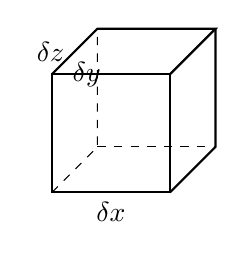
\begin{tikzpicture}[scale=1.5, >=stealth]
    % Cube
    \draw[thick] (0,0,0) -- (1,0,0) node[midway, below] {$\delta x$} -- (1,1,0) -- (0,1,0) node[midway, left] {$\delta y$} -- cycle;
    \draw[thick] (0,1,0) -- (0,1,-1) node[midway, left] {$\delta z$} -- (1,1,-1) -- (1,1,0);
    \draw[thick] (1,0,0) -- (1,0,-1) -- (1,1,-1);
    \draw[dashed] (0,0,0) -- (0,0,-1) -- (0,1,-1);
    \draw[dashed] (0,0,-1) -- (1,0,-1);
\end{tikzpicture}
\end{center}

Deformation $\leftrightarrow$ Linear deformations:

\begin{center}
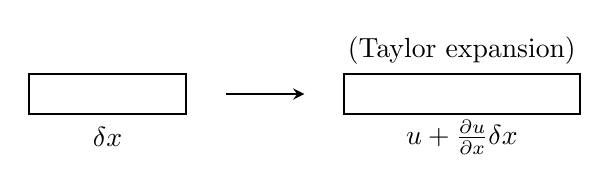
\begin{tikzpicture}[>=stealth]
    \draw[thick] (0,0) rectangle (2,0.5);
    \node at (1, -0.3) {$\delta x$};
    
    \draw[->, thick] (2.5, 0.25) -- (3.5, 0.25);
    
    \draw[thick] (4,0) rectangle (7,0.5);
    \node at (5.5, -0.3) {$u + \frac{\partial u}{\partial x} \delta x$};
    \node at (5.5, 0.8) {(Taylor expansion)};
\end{tikzpicture}
\end{center}

$$ \frac{d(\delta x)}{dt} = \frac{\partial u}{\partial x} \delta x \implies \frac{1}{\delta x} \frac{d(\delta x)}{dt} = \frac{\partial u}{\partial x} $$

Also: 
\begin{itemize}
    \item $\frac{\partial v}{\partial y}$: linear deformation in $y$
    \item $\frac{\partial w}{\partial z}$: linear deformation in $z$
\end{itemize}

\textbf{Volume change:} $\delta V = \delta x \delta y \delta z$
$$ \frac{1}{\delta V} \frac{d(\delta V)}{dt} = \frac{1}{\delta x} \frac{d(\delta x)}{dt} + \frac{1}{\delta y} \frac{d(\delta y)}{dt} + \frac{1}{\delta z} \frac{d(\delta z)}{dt} = \frac{\partial u}{\partial x} + \frac{\partial v}{\partial y} + \frac{\partial w}{\partial z} = \nabla \cdot \vec{v} $$
If $\rho = \text{cte}$ (incompressible), then $\nabla \cdot \vec{v} = 0$.

\subsubsection{Angular Deformation}

\begin{center}
\begin{tikzpicture}[scale=2, >=stealth]
    % Original Element
    \draw[dashed] (0,0) rectangle (1,1);
    \node at (0.5, -0.2) {$\delta x$};
    \node at (-0.2, 0.5) {$\delta y$};
    
    % Deformed Element
    \draw[thick, primary] (0,0) -- (1, 0.2) -- (0.8, 1.2) -- (-0.2, 1) -- cycle;
    
    % Angles
    \draw[->] (0.3, 0) arc (0:11.3:0.3);
    \node at (0.4, 0.1) {$\delta \alpha$};
    
    \draw[->] (0, 0.3) arc (90:101.3:0.3);
    \node at (-0.1, 0.4) {$\delta \beta$};
    
    % Velocities
    \draw[->, thick, accent] (1,0) -- (1,0.2) node[right] {$\frac{\partial v}{\partial x} \delta x \Delta t$};
    \node at (1.1, 0) {$A$};
    \node at (0, 1.1) {$B$};
\end{tikzpicture}
\end{center}

Angular velocity of segment $OA$:
$$ \omega_{OA} = \lim_{\Delta t \to 0} \frac{\delta \alpha}{\Delta t} = \lim_{\Delta t \to 0} \frac{1}{\Delta t} \left( \frac{(\frac{\partial v}{\partial x} \delta x) \Delta t}{\delta x} \right) = \frac{\partial v}{\partial x} $$

Similarly for segment $OB$ (clockwise):
$$ \omega_{OB} = -\frac{\partial u}{\partial y} $$

Average rotation (Rotation of the bisector line):
$$ \omega_z = \frac{1}{2} (\omega_{OA} + \omega_{OB}) = \frac{1}{2} \left( \frac{\partial v}{\partial x} - \frac{\partial u}{\partial y} \right) $$

Similarly for the other axes:
$$ \omega_x = \frac{1}{2} \left( \frac{\partial w}{\partial y} - \frac{\partial v}{\partial z} \right), \quad \omega_y = \frac{1}{2} \left( \frac{\partial u}{\partial z} - \frac{\partial w}{\partial x} \right) $$

Angular velocity vector:
$$ \vec{\omega} = \omega_x \hat{i} + \omega_y \hat{j} + \omega_z \hat{k} = \frac{1}{2} \nabla \times \vec{v} $$

\begin{defbox}{Vorticity}
The vorticity $\vec{\zeta}$ is defined as twice the angular velocity:
$$ \vec{\zeta} = \nabla \times \vec{v} = \text{curl } \vec{v} $$
\end{defbox}

\subsubsection{Circulation}

\begin{center}
\begin{tikzpicture}
    % Curve
    \draw[thick, fill=gray!20, decoration={random steps,segment length=3mm,amplitude=1mm}, decorate] (0,0) ellipse (2cm and 1cm);
    \node at (0,0) {$A$};
    \node at (2.2, 0.5) {$C$};
    
    % Vectors
    \draw[->, thick, primary] (1.4, 0.7) -- (0.8, 0.9) node[above] {$d\vec{s}$};
    \draw[->, thick, accent] (1.4, 0.7) -- (1.8, 1.2) node[right] {$\vec{v}$};
    
    \node at (0,-1.5) {Counter-clockwise path (Right-hand rule)};
\end{tikzpicture}
\end{center}

Vorticity integrated over the Area gives Circulation $\Gamma$:
$$ \Gamma = \oint_C \vec{v} \cdot d\vec{s} \underset{\text{Stokes}}{=} \int_A (\nabla \times \vec{v}) \cdot d\vec{A} $$

\textbf{Show: Inviscid flow $\implies$ No change in rotation (Kelvin's Circulation Theorem)}

$$ \frac{D\Gamma}{Dt} = \frac{d\Gamma}{dt} = \frac{d}{dt} \oint_C \vec{v} \cdot d\vec{s} = \oint_C \frac{d\vec{v}}{dt} \cdot d\vec{s} $$
$$ = \oint_C \left[ \frac{\partial \vec{v}}{\partial t} + \vec{v} \cdot \nabla \vec{v} \right] \cdot d\vec{s} $$

Using Navier-Stokes for inviscid flow ($\mu \to 0$):
$$ \implies \frac{D\Gamma}{Dt} = \oint_C \frac{1}{\rho} (-\nabla p + \rho \vec{g}) \cdot d\vec{s} $$
Since $\rho \vec{g} = -\rho g \hat{k} = \nabla(-\rho g z)$:
$$ = \oint_C \nabla \left( \frac{-p - \rho g z}{\rho} \right) \cdot d\vec{s} $$

By Stokes' Theorem:
$$ \oint_C \nabla \phi \cdot d\vec{s} = \int_A \nabla \times (\nabla \phi) \cdot d\vec{A} = 0 \quad (\text{since } \nabla \times \nabla \phi = \vec{0}) $$
$$ \implies \frac{d\Gamma}{dt} = 0 \quad (\text{for inviscid flow, } \Gamma \text{ is conserved}) $$

Because the curve $C$ is arbitrary, for the vorticity:
\textbf{An inviscid flow with initially zero vorticity ($\nabla \times \vec{v} = \vec{0}$) remains irrotational.}

\textbf{Q: How is vorticity generated in a flow?}
$\implies$ Wall with no-slip boundary condition!

\begin{center}
\begin{tikzpicture}[>=stealth]
    % Wall
    \draw[thick] (0,0) -- (4,0);
    \fill[pattern=north east lines] (0,-0.2) rectangle (4,0);
    \node[below] at (2,-0.2) {Wall (No-slip BC)};
    
    % Velocity Profile
    \draw[->, thick, primary] (0,0) -- (0,0);
    \draw[->, thick, primary] (0,0.5) -- (1,0.5);
    \draw[->, thick, primary] (0,1.0) -- (1.8,1.0);
    \draw[->, thick, primary] (0,1.5) -- (2.4,1.5);
    \draw[->, thick, primary] (0,2.0) -- (2.8,2.0);
    
    % Profile Curve
    \draw[dashed, thick, accent] (0,0) .. controls (1.9, 0.8) and (2.7, 1.8) .. (2.8, 2.0);
    
    \node[right] at (2.5, 1.0) {$\frac{\partial u}{\partial y} \neq 0 \implies \text{Vorticity generation}$};
\end{tikzpicture}
\end{center}